% 2008 年天津卷理科第 19 题：四棱锥 P-ABCD，底面 ABCD 是矩形，
%   AB=3，AD=2，PA=2，PD=2√2，∠PAB=60°。
% 来源 PDF：gaokaomath-src/普通高考/2008/2008天津理.pdf
% SHA-256：e2442be3c0179c888e74b31dda58e749b6ab84ac8cccf86eae4677ab3843f48b
% 原页：2008天津理.pdf 第 1 页（A3 三栏）第 3 栏，书页码 487。
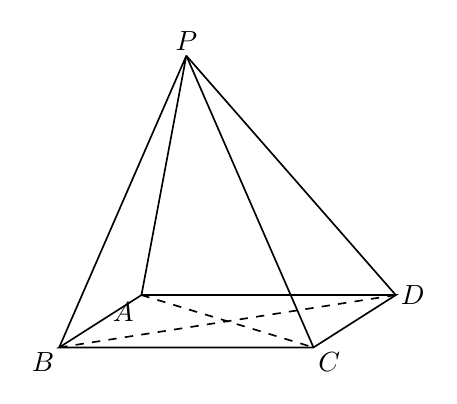
\begin{tikzpicture}[scale=0.95, semithick,
  every node/.style={inner sep=1.5pt}]
  \coordinate (A) at (1.1,0.9);
  \coordinate (B) at (0.0,0.2);
  \coordinate (C) at (3.4,0.2);
  \coordinate (D) at (4.5,0.9);
  \coordinate (P) at (1.7,4.1);

  \draw (A) -- (B) -- (C) -- (D) -- cycle;
  \draw (P) -- (A);
  \draw (P) -- (B);
  \draw (P) -- (C);
  \draw (P) -- (D);
  \draw[dashed] (B) -- (D);
  \draw[dashed] (A) -- (C);

  \node[below left=1pt] at (A) {$A$};
  \node[below left] at (B) {$B$};
  \node[below right] at (C) {$C$};
  \node[right] at (D) {$D$};
  \node[above] at (P) {$P$};
\end{tikzpicture}
